\chapter{Ergebnisse}
\label{kap:ergebnisse}

In den \abbn~\ref{fig:clamp_8} bis \ref{fig:clamp_4_5} wurde die Anzahl zum Zeitpunkt $t$ intakter \amide~gegenüber ihrer Überlebensdauern bei verschiedenen pH-Werten halblogarithmisch aufgetragen. Tabelle~\ref{tab:zuordnung_ph_abbildungen} zeigt welche Daten bei welchen pH-Werten aufgenommen wurden.

% Tabelle: Zuordnung von pH-Werten und entsprechenden Abbdilungen
\begin{table}[h]
	\centering
	\caption[Zuordnung von pH-Werten und den dazugehörigen Abbildungen]{Zuordnung von pH-Werten und den dazugehörigen Abbildungen}
	\label{tab:zuordnung_ph_abbildungen}
	\begin{threeparttable}
		\keepXColumns
		\begin{tabularx}{\textwidth}{X X X X}
			\textbf{pH-Wert}	&	\textbf{Abbildungen}	&	\textbf{Anzahl der ausgewerteten Kraftkurven}	&	\textbf{Anzahl aller aufgenommenen Kraftkurven}\\
			\toprule
			\toprule
			8	&	\ref{fig:clamp_8}	&	14	&	155\\
			7,4	&	\ref{fig:clamp_7_4}	&	16	&	360\\
			4,5	&	\ref{fig:clamp_4_5}	&	11	&	41\\
			\toprule
			\toprule
		\end{tabularx}
	\end{threeparttable}
\end{table}

Bei den pH-Werten 8 und 7,4 (\abbn~\ref{fig:clamp_8} und \ref{fig:clamp_7_4}) sind deutlich zwei Prozesse anhand der unterschiedlichen Steigungen zu erkennen. In dem pH-Wert von 4,5 (\abb~\ref{fig:clamp_4_5}) war dieser Zusammenhang nicht mehr klar erkennbar. Es wurden alle Force-Clamp-Experimente durch einen biexponentiellen Zerfall nach Gleichung~\ref{eq:biexponentieller_zerfall} ausgewertet.\\
Die, durch den Fit des biexponentiellen Zerfalls erhaltenen Parameter sind in Tabelle~\ref{tab:parameter_biexponentieller_zerfall} zusammengefasst. Zusätzlich wurden die zu den Geschwindigkeitskonstanten $k_i$ korrespondierenden Zeitkonstanten $\tau_i$, sowie der Mischungskoeffizient $A$ angegeben. Die Fehlerintervalle der Fitparameter betrugen jeweils $\pm$ eine Standardabweichung\footnote{Die von Igor Pro angegebenen Unsicherheit der Parameter entspricht dem Ergebnis, wenn die Anpassung des biexponentiellen Zerfalls in hoher Anzahl an dieselben Daten mit jeweils unterschiedlichem Rauschen durchgeführt werden würden. Die angegebene Unsicherheit ist damit die Standardabweichung des Mittelwerts jedes Parameters, aus dieser häufig hintereinander durchgeführten Regressionsrechnung.}.

% Modellparameter des biexponentiellen Zerfalls
\begin{table}[h]
	\centering
	\caption[Modellparameter des biexponentiellen Zerfalls]{Modellparameter des biexponentiellen Zerfalls in Abhängigkeit des pH-Wertes. Die zu den Geschwindigkeitskonstanten $k_i$ korrespondierenden Zeitkonstanten $\tau_i$ wurden ebenfalls mit angegeben. Die Fehlerintervalle lagen jeweils $\pm$ eine Standardabweichung um den entsprechenden Parameter.}
	\label{tab:parameter_biexponentieller_zerfall}
	\begin{threeparttable}
		\keepXColumns
		\begin{tabularx}{\textwidth}{p{2cm} X X X X X}
			\textbf{pH-Wert}	&	\textbf{$k_1~/~s^{-1}$}	&	\textbf{$\tau_1~/~s$}	&	\textbf{$k_2~/~s^{-1}$}	&	\textbf{$\tau_2~/~s$}	&	\textbf{$A$}\\
			\toprule
			\toprule
			8	& $5,3 \pm 1,17$	&	$0,19 \pm 0,083$	&	$0,12 \pm 0,018$	&	$~8,33 \pm 2,500$	&	$0,35 \pm 0,036$	\\
			7,4	&	$4,1 \pm 0,67$	&	$0,24 \pm 0,079$	&	$0,06 \pm 0,007$	&	$18,18 \pm 3,889$	&	$0,44 \pm 0,025$	\\
			4,5	&	$2,7 \pm 1,55$	&	$0,37 \pm 0,425$	&	$0,08 \pm 0,008$	&	$13,33 \pm 2,500$	&	$0,19 \pm 0,044$	\\	
			\toprule
			\toprule
		\end{tabularx}
	\end{threeparttable}
\end{table}

Die angegebenen Werte für die schnellen Prozesse ($k_1$) der pH-Werte von 8, 7,4 und 4,5 ($k_1^8 = 5,3~s^{-1} \pm 1,17~s^{-1}$, $k_1^{7,4} = 4,1~s^{-1} \pm 0,67~s^{-1}$ und $k_1^{4,5} = 2,7~s^{-1} \pm 1,55~s^{-1}$), überschnitten sich in ihren Fehlerintervallen. Verglichen mit dem Fehlerintervall $\Delta k_1^8 = 0,67~s^{-1}$ (8 gemessene Überlebenszeiten) lagen die Fehlerintervalle der beiden anderen Geschwindigkeitskonstanten ($\Delta k_1^{7,4} = 1,17~s^{-1}$ mit 5 gemessenen Überlebenszeiten und $\Delta k_1^{4,5} = 1,55~s^{-1}$ mit 2 gemessenen Überlebenszeiten) um eine Größenordnung höher. er Wert für $k_1^{7,4} = 4,1~s^{-1}$ war daher robuster als für $k_1^8$ bzw. $k_1^{4,5}$.\\
Der Wert für $k_1^{4,5}$ war als problematisch zu betrachten, da in diesen Prozess lediglich 2 Überlebenszeiten fielen (vgl. \abb~\ref{fig:clamp_4_5}). Dadurch war der schnelle Prozess nicht klar definiert  und $k_1^{4,5}$ hatte keine sinnvolle Aussagekraft.\\
Die mittlere Lebensdauern der schnellen Prozesse lagen unterhalb einer Sekunde ($\tau_1^8 = 0,19~s \pm 0,083~s$, $\tau_1^{7,4} = 0,24~s \pm 0,079~s$ und $\tau_1^{4,5} = 0,37~s \pm 0,425~s$). Insbesondere der Wert $\tau_1^{4,5}$ war analog zu $k_1^{4,5}$ nicht aussagekräftig.\\
Für die langsamen Prozesse ($k_2$) ergab sich das Gegenteil. Die Werte für $k_2^{7,4} = 0,06~s^{-1} \pm 0,007~s^{-1}$ bzw. $k_2^{4,5} = 0,08~s^{-1} \pm 0,008~s^{-1}$ waren eine Größenordnung kleiner als $k_2^8 = 0,12~s^{-1} \pm 0,018~s^{-1}$. Die mittleren Lebensdauern der langsamen Prozesse lagen zwischen 8 und 19 Sekunden ($\tau_2^8 = 8,33~s \pm 2,5~s$, $\tau_2^{7,4} = 18,18~s \pm 3,889~s$ und $\tau_2^{4,5} = 13,33~s \pm 2,5~s$).\\
Der Mischungskoeffizient $A$ gab die Verteilung der Datenpunkte auf den schnellen und langsamen Prozess innerhalb des jeweiligen Experiments an. Dabei fielen bei pH 8 mit $A = 0,35$ ca. 5 Überlebenszeiten in den schnellen Prozess und mit $(1-A) = 0,65$ ca. 9 Überlebenszeiten in den langsamen Prozess (vgl. \abb~\ref{fig:clamp_8}). Die große Unsicherheit im Fitparameter $k_1^8$ mit $\Delta k_1^8 = \pm 1,84~s^{-1}$ kam daher, dass für den Fit des biexponentiellen Zerfalls zu wenig Überlebenszeiten in den schnellen Prozess fielen.\\
Bei pH 7,4 fielen mit $A = 0,44$ ca. 7 Überlebenszeiten in den schnellen Prozess und mit $(1-A) = 0,56$ ca. 9 Überlebenszeiten in den langsamen Prozess (vgl. \abb~\ref{fig:clamp_7_4}). Hier waren für beide Prozesse ausreichend Datenpunkte vorhanden, sodass $A = 0,44$ nahe bei dem Wert 0,5 lag. Die Fehler der Fitparameter sind daher eine Größenordnung kleiner als die Werte der Fitparameter selbst.\\
Bei pH 4,5 fielen mit $A = 0,19$ ca. 2 Überlebenszeiten in den schnellen Prozess und mit $(1-A) = 0,81$ ca. 9 Überlebenszeiten in den langsamen Prozess (vgl. \abb~\ref{fig:clamp_4_5}). Die zwei Überlebenszeiten im schnellen Prozess waren jedoch zu wenig für eine klare Aussage darüber, ob für pH 4,5 die Annahme eines schnellen Prozesses sinnvoll war. Wurde alle Überlebenszeiten bei pH 4,5 als ein Prozess betrachtet\footnote{Einfacher, exponentieller Zerfall mit A bei 1 fixiert.}, ergab sich $k^{4,5} = 0,11~s^{-1} \pm 0,010~s^{-1}$. Damit passte dieser Prozess in der Größenordnung zu $k_2^8 = 0,12~s^{-1}$. 

% Ergebnisse Clamp pH8
\begin{figure}[H]
	\centering
	\scalebox{0.9}{
		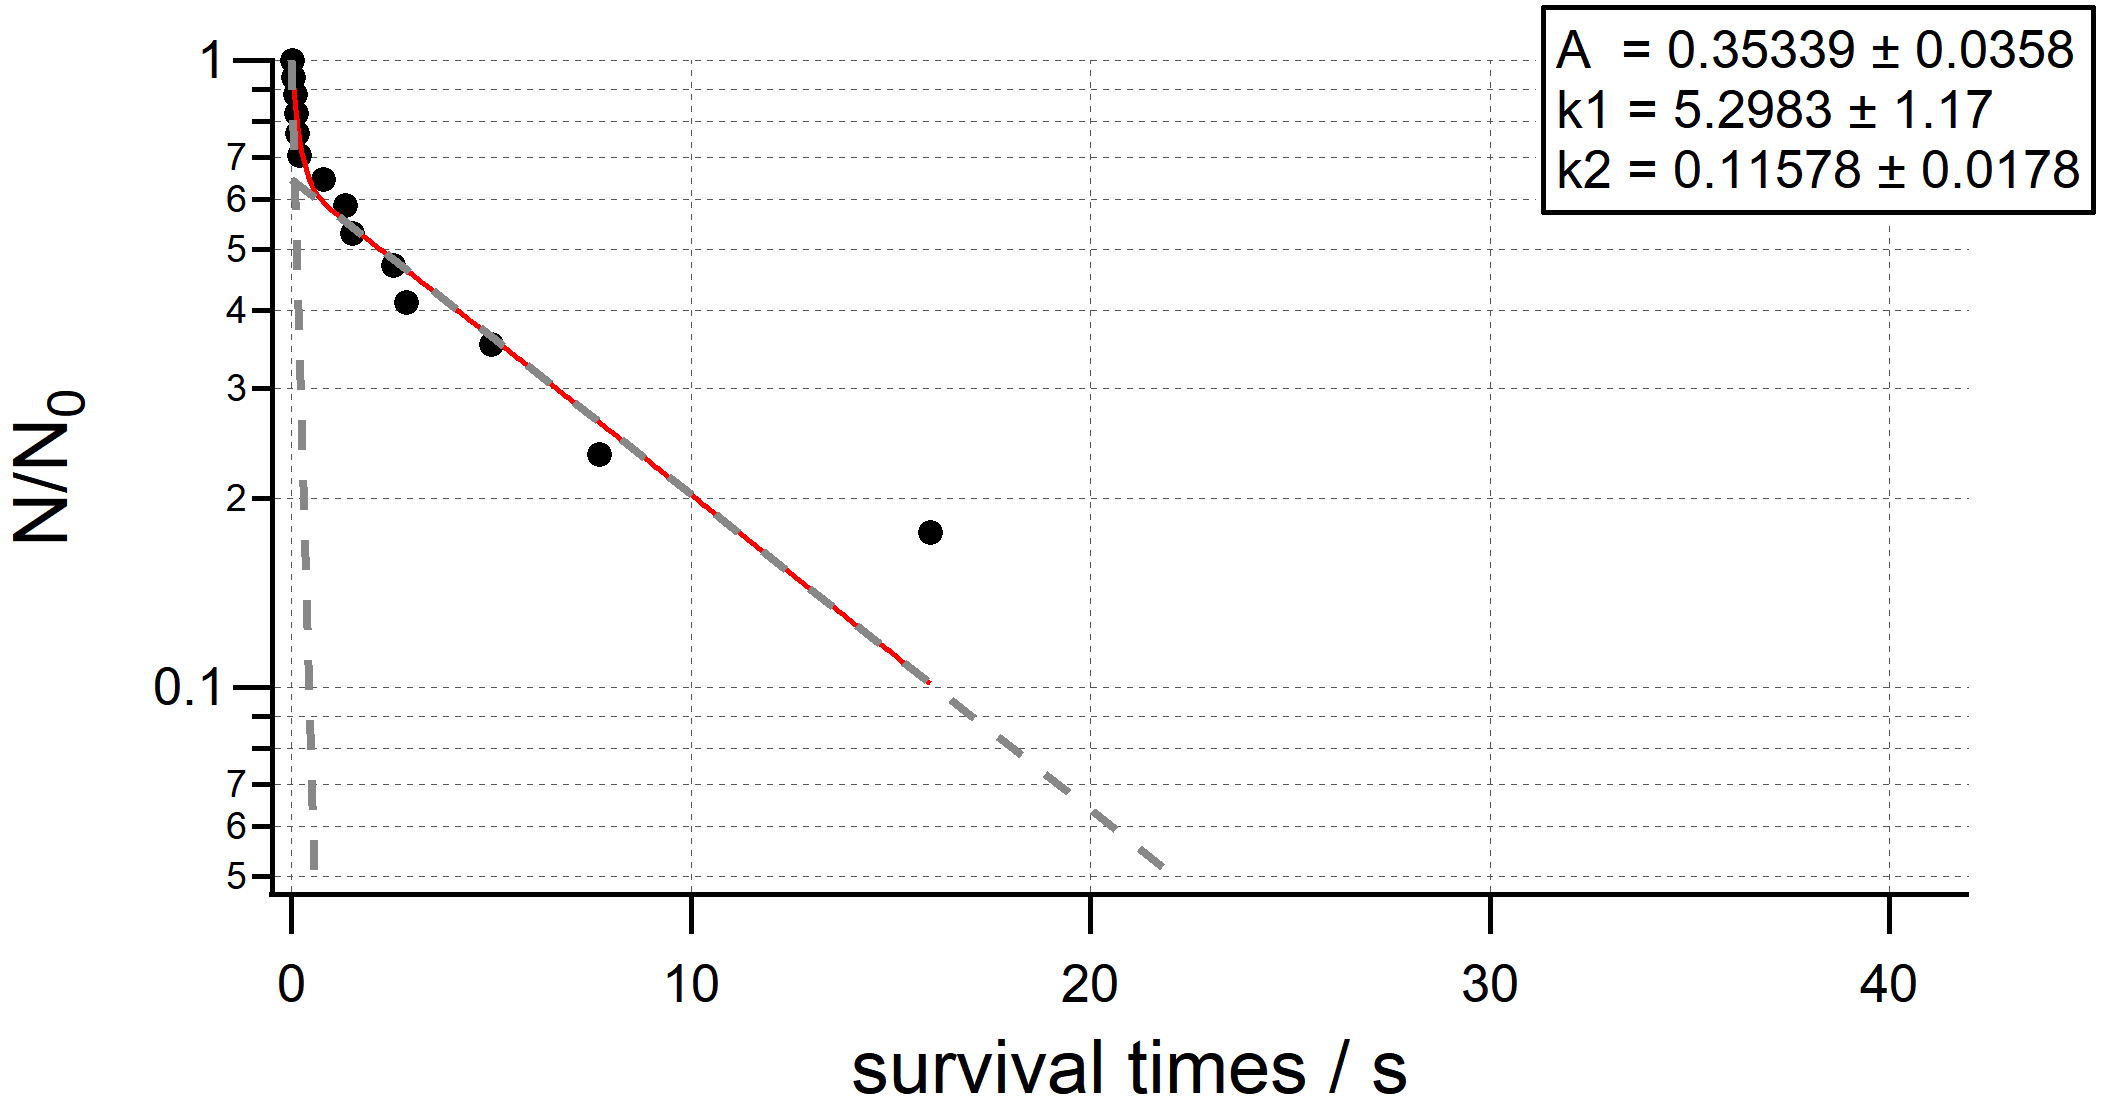
\includegraphics[width=\linewidth]{Abbildungen/clamp_ph_8_multiple_ruptures.png}
	} % scalebox
	\caption[Ergebnisse der Force-Clamp-Experimente bei einem pH-Wert von 8]{Ergebnisse der Force-Clamp-Experimente bei einem pH-Wert von 8. Es konnten zwei Zerfallsprozesse beobachtet werden. Die Geschwindigkeitskonstante (grau gestrichelte Linien) $k_1~=~5,3~s^{-1}~\pm~1,84~s^{-1}$ und $k_2~=~0,12~s^{-1}~\pm~0,018~s^{-1}$, sowie der Mischungskoeffizient beider Prozesse $A~=~0,35~\pm~0,036$ konnten durch die Anpassung eines biexponentiellen Zerfalls an die Daten ermittelt werden. Für diese Auswertung wurden insgesamt 14 Clampereignisse verwendet.}
	\label{fig:clamp_8}
\end{figure}


% Ergebnisse Clamp pH7,4
\begin{figure}[H]
	\centering
	\scalebox{0.9}{
		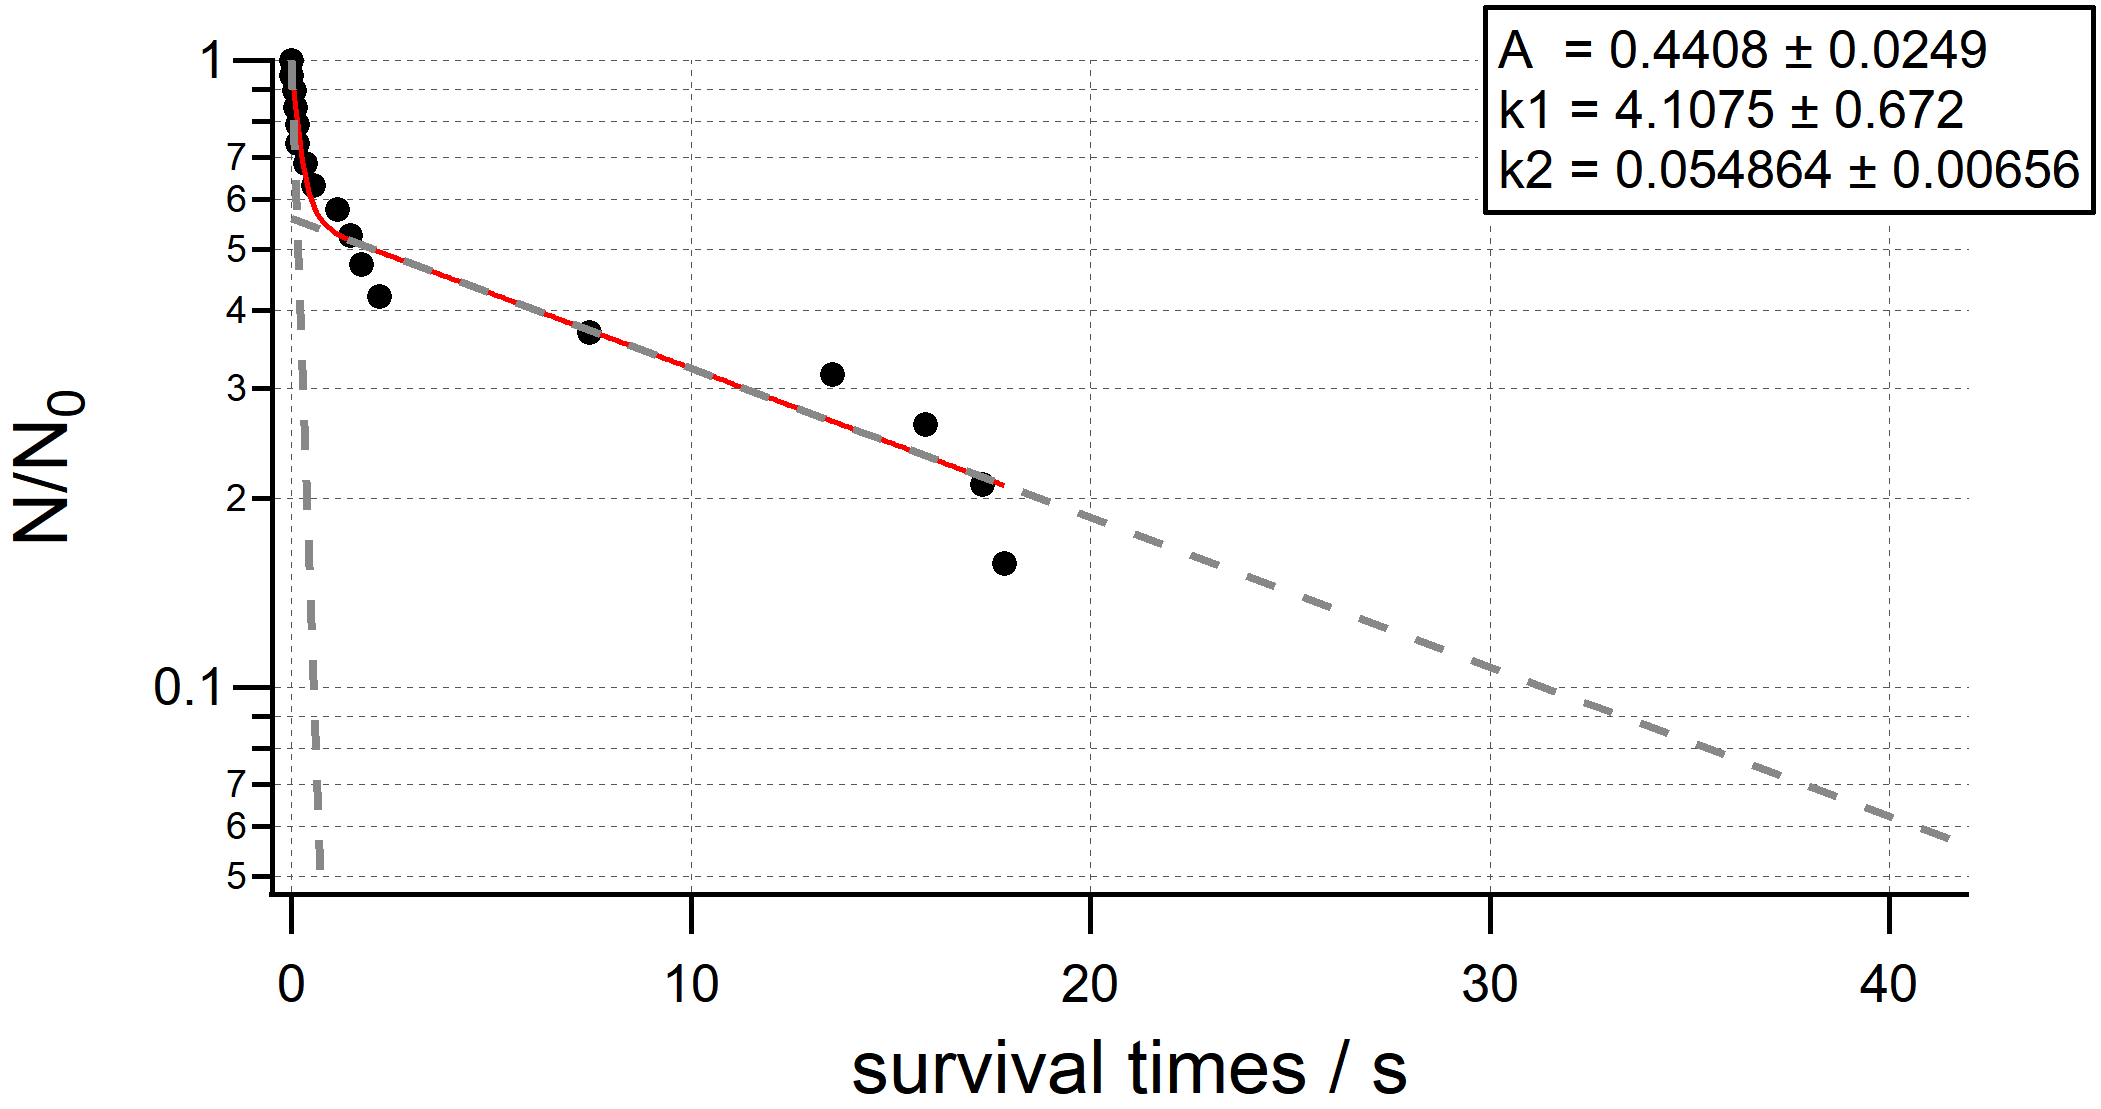
\includegraphics[width=\linewidth]{Abbildungen/clamp_ph7_4_multiple_ruptures.png}
	} % scalebox
	\caption[Ergebnisse der Force-Clamp-Versuche bei einem pH-Wert von 7,4]{Ergebnisse der Force-Clamp-Versuche bei einem pH-Wert von 7,4.  Es konnten zwei Zerfallsprozesse beobachtet werden. Die Geschwindigkeitskonstante (grau gestrichelte Linien) $k_1~=~4,1~s^{-1}~\pm~0,67~s^{-1}$ und $k_2~=~0,055~s^{-1}~\pm~0,0066~s^{-1}$, sowie der Mischungskoeffizient beider Prozesse $A~=~0,44~\pm~0,025$ konnten durch die Anpassung eines biexponentiellen Zerfalls an die Daten ermittelt werden. Für diese Auswertung wurden insgesamt 16 Clampereignisse verwendet.}
	\label{fig:clamp_7_4}
\end{figure}

% Ergebnisse Clamp pH4,5
\begin{figure}[H]
	\centering
	\scalebox{0.9}{
		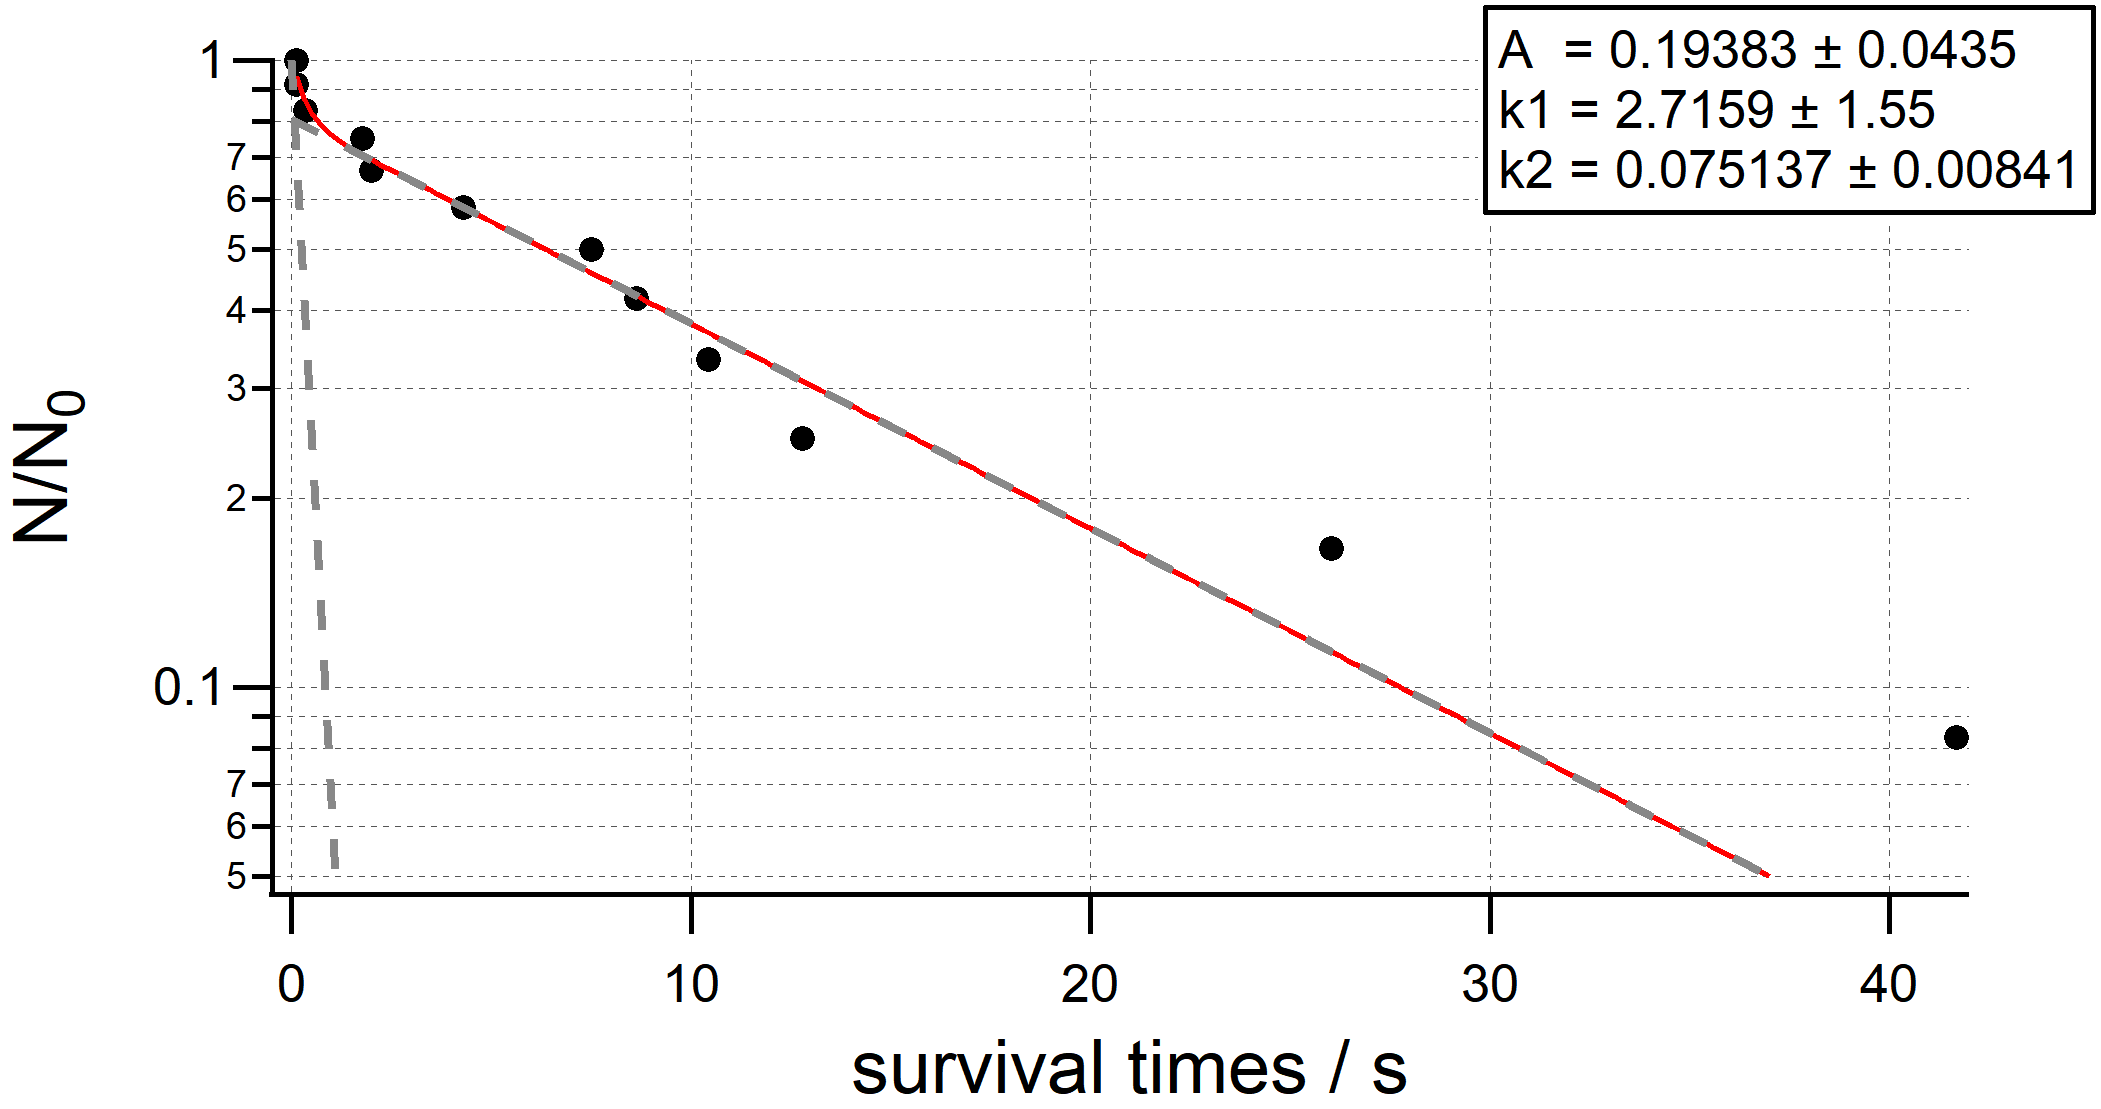
\includegraphics[width=\linewidth]{Abbildungen/clamp_ph4_5_multiple_ruptures.png}
	} % scalebox
	\caption[Ergebnisse der Force-Clamp-Versuche bei einem pH-Wert von 4,5]{Ergebnisse der Force-Clamp-Versuche bei einem pH-Wert von 4,5. Es konnten zwei Zerfallsprozesse beobachtet werden. Die Geschwindigkeitskonstante (grau gestrichelte Linien) $k_1~=~2,7~s^{-1}~\pm~1,55~s^{-1}$ und $k_2~=~0,075~s^{-1}~\pm~0,0084~s^{-1}$, sowie der Mischungskoeffizient beider Prozesse $A~=~0,19~\pm~0,044$ konnten durch die Anpassung eines biexponentiellen Zerfalls an die Daten ermittelt werden. Für diese Auswertung wurden insgesamt 11 Clampereignisse verwendet.}
	\label{fig:clamp_4_5}
\end{figure}

In \abb~\ref{fig:general_curve_composition} wurde die kategorische Zusammensetzung aller aufgenommenen Kraftkurven der jeweiligen pH-Werte aufgeschlüsselt. Zur Auswertung wurden ausschließlich Kraftkurven aus den Kategorien A und B, ohne zusätzliche Bemerkungen herangezogen. Diese beiden Kategorien stellten die Ausbeute der Force-Clamp-Experimente dar (grüne und blaue Bereiche in \abb~\ref{fig:general_curve_composition}). Die Ausbeute ergab 9\% für pH 8, 5\% für pH 7,4 und 29\% für pH 4,5. Tabelle~\ref{tab:general_curve_composition} verdeutlicht diesen Sachverhalt. Das Verhältnis von Kategorie A zu Kategorie B Kurven kurz $A/B$, lag für pH 4,5 bei 0,32. Im Vergleich zu den anderen pH-Werten ($A/B^{7,4} = 4$ bzw. $A/B^{8} = 1,25$) sehr weit unterhalb von 1. Für die Auswertung der Force-Clamp-Experimente bei pH 4,5 standen demnach hauptsächlich Kategorie B kurven zur Verfügung. Bei den pH-Werten 8 und 7,4 hingegen standen hauptsächlich Kategorie A zur Verfügung. Das vermehrte Auftreten von Kategorie B Kurven bei dem pH-Wert von 4,5 verglichen mit den pH-Werten von 8 und 7,4 deutete auf eine höhere Interaktion zwischen \spitze~dem \spacer~und dem Substrat hin.

% General Curve Composition
\begin{figure}[H]
	\centering
	\scalebox{0.9}{
		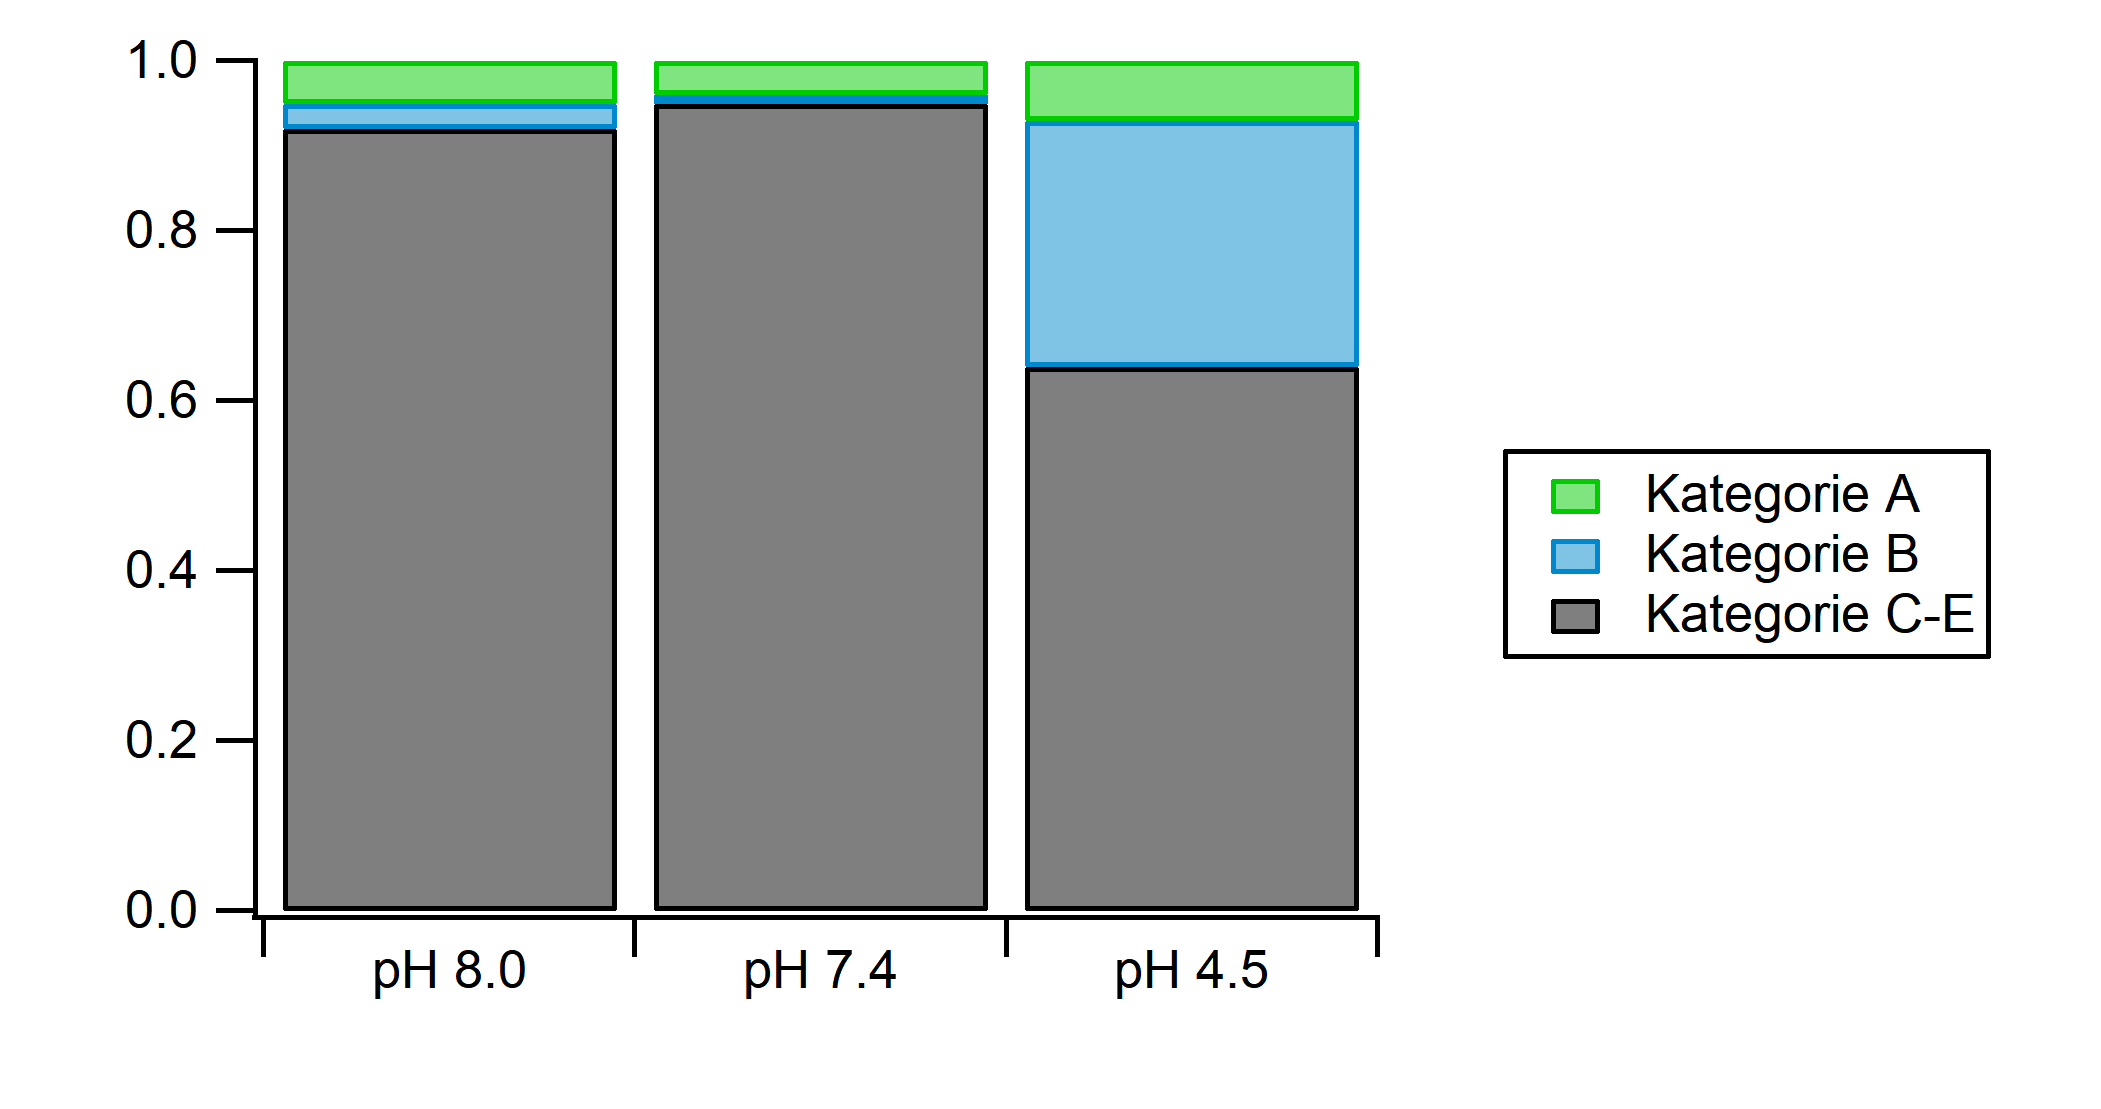
\includegraphics[width=\linewidth]{Abbildungen/curve_composition_multiple_ruptures.png}
	} % scalebox
	\caption[Kategorische Zusammensetzung aller aufgenommenen Kraftkurven]{Kategorische Zusammensetzung aller aufgenommenen Kraftkurven der Experimente bei den pH-Werten 8, 7,4 und 4,5. Kategorie A (pH = 8): 5\%. Kategorie B (pH = 8): 3\%. Kategorie C-E (pH = 8): 91\%. Kategorie A (pH = 7,4): 4\%. Kategorie B (pH = 7,4): 1\%. Kategorie C-E (pH = 7,4): 95\%. Kategorie A (pH = 4,5): 7\%. Kategorie B (pH = 4,5): 29\%. Kategorie C-E (pH = 4,5): 64\%. $N_8$ = 155, $N_{7,4}$ = 360, $N_{4,5}$ = 41.}
	\label{fig:general_curve_composition}
\end{figure}

% Zusammensetzung und Ausbeute der Force-Clamp-Experimente
\begin{table}[H]
	\centering
	\caption[Kategorische Zusammensetzung aller ausgewerteten Clampereignisse]{Kategorische Zusammensetzung aller ausgewerteten Clampereignisse bei unterschiedlichen pH-Werten.}
	\label{tab:general_curve_composition}
	\begin{threeparttable}
		\keepXColumns
		\begin{tabularx}{\textwidth}{X X X X}
			\textbf{pH-Wert}	&	\textbf{Kategorie A /\%}	&	\textbf{Kategorie B /\%}	&	\textbf{Kategorie C-E/\%}	\\
			\toprule
			\toprule
			8	&	5	&	4	&	91	\\
			7,4	&	4	&	1	&	95	\\
			4,5	&	7	&	22	&	71	\\
			\toprule
			\toprule
		\end{tabularx}
	\end{threeparttable}
\end{table}

Ein ähnliches Bild ergab sich bei den verworfenen Kraftkurven (Kategorie C-E). In \abb~\ref{fig:discarded_curve_composition} wurden ausschließlich die verworfenen Kraftkurve bei den verschiedenen pH-Werten nach Kategorien aufgeschlüsselt. Kraftkurven aus den Kategorien C und D konnten keiner Einzelmolekülinteraktion zugeordnet werden, zeigten jedoch deutliche Mehrfach- oder überlagerte Mehrfachabrisse. Kraftkurven der Kategorie E zeigten keinerlei molekülspezifische Interaktionen zwischen Substrat und \spitze~(s. Abschnitt~\ref{subsec:kategorisierung_der_kraftkurven}). Tabelle~\ref{tab:discarded_curve_composition} fast die kategorische Aufschlüsselung aus \abb~\ref{fig:discarded_curve_composition} Zusammen. Kategorie C Kurven erschienen ausschließlich bei pH 8 und wurden nicht weiter berücksichtigt. Die Zusammensetzung der verworfenen Kraftkurven zeigte eine Zunahme von Kategorie D Kurven bei pH 4,5. Das Verhältnis von Kategorie C zu D Kurven lag bei pH 4,5 ($C/D^{4,5} = 0,69$) mehr als doppelt so hoch wie bei den anderen pH-Werten ($C/D^{8} = 0,33$ und $C/D^{7,4} = 0,25$). Dies passte zur Aussage von \abb~\ref{fig:general_curve_composition}, denn auch in den verworfenen Kraftkurven zeigte sich bei pH 4,5 eine erhöhte Interaktion.

% Discarded Curve Composition
\begin{figure}[H]
	\centering
	\scalebox{0.9}{
		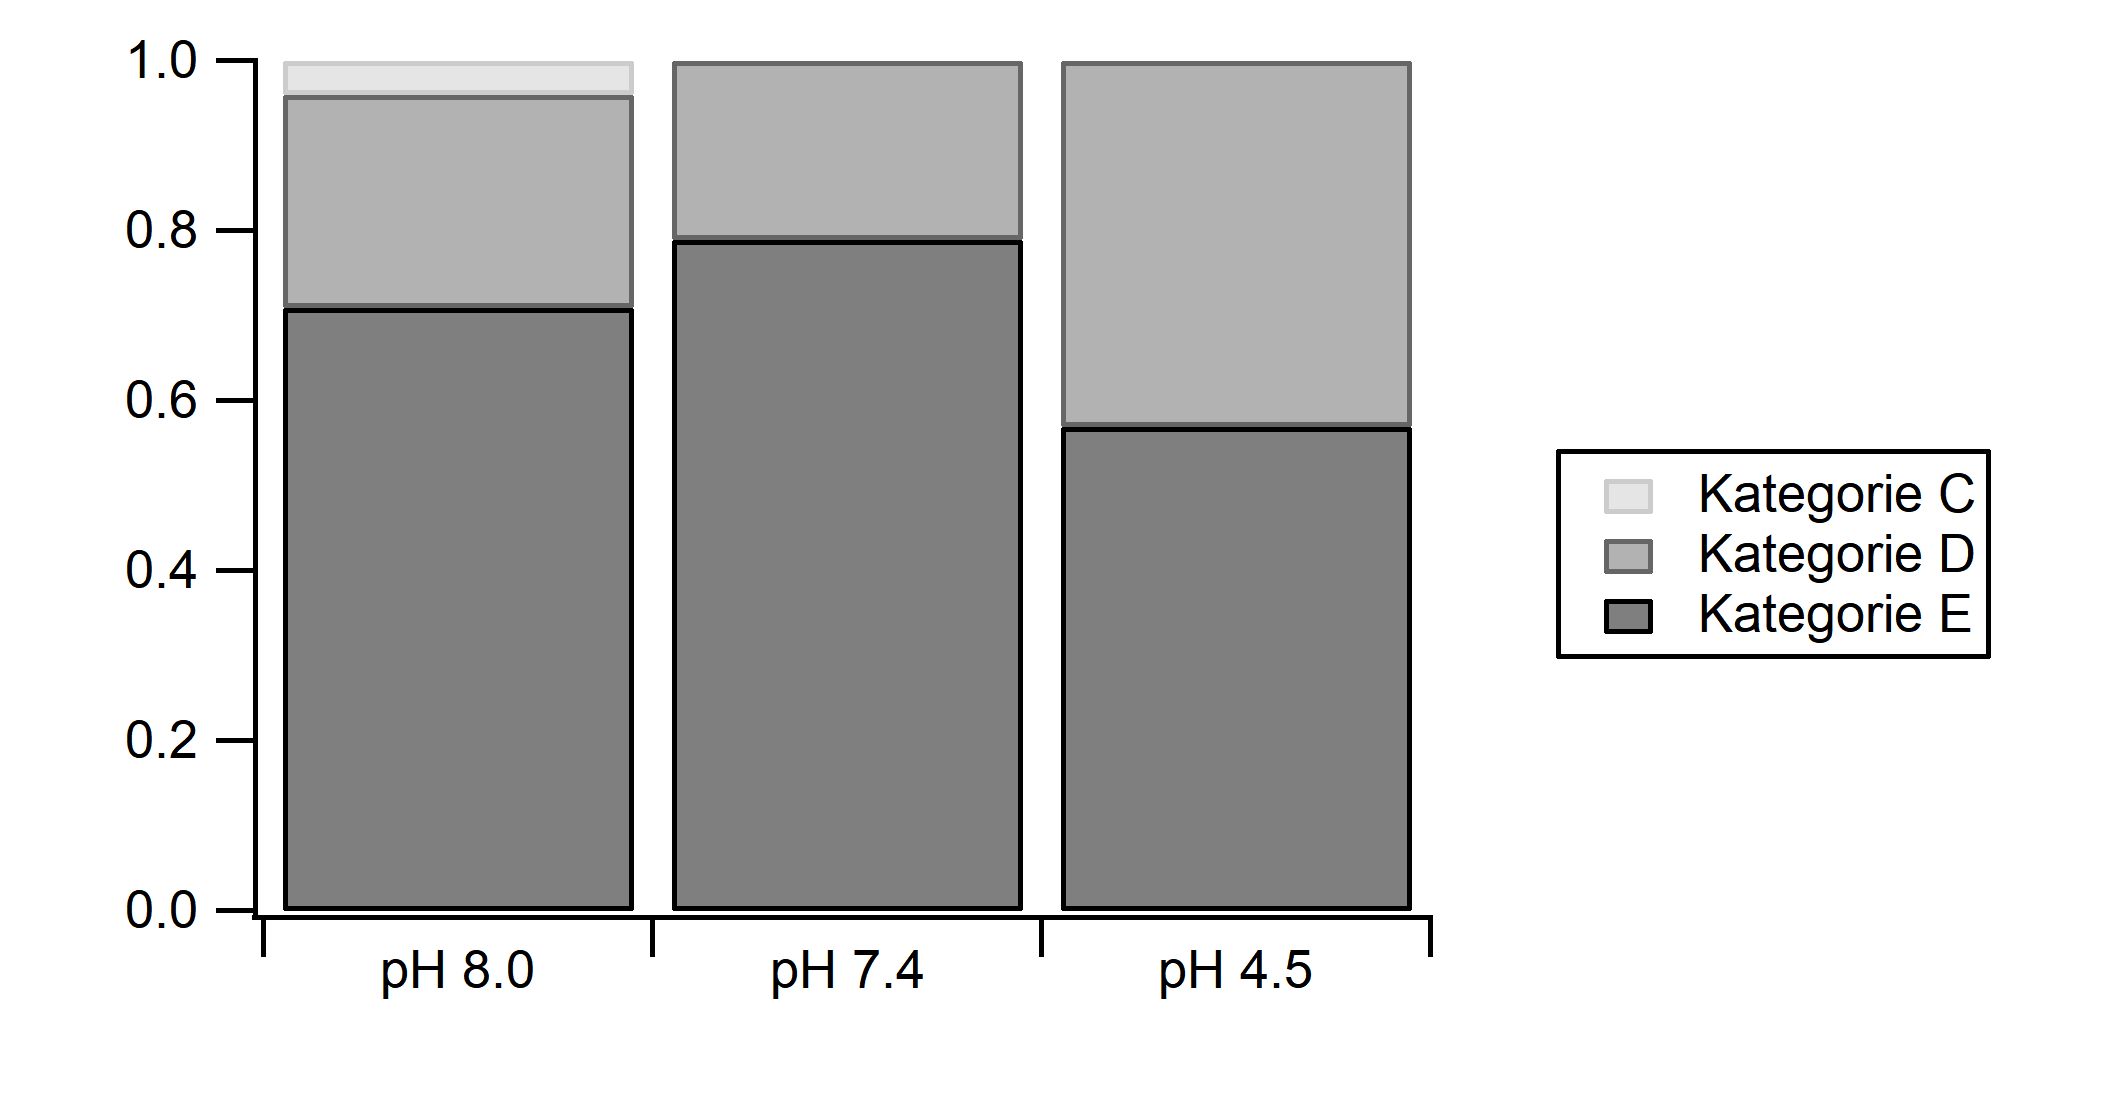
\includegraphics[width=\linewidth]{Abbildungen/discarded_curve_composition_multiple_ruptures.png}
	} % scalebox
	\caption[Kategorische Zusammensetzung aller verworfenen Kraftkurven]{Kategorische Zusammensetzung aller verworfenen Kraftkurven der Experimente bei den pH-Werten 8, 7,4 und 4,5. Kategorie C (pH = 8): 4\%. Kategorie D (pH = 8): 25\%. Kategorie E (pH = 8): 71\%. Kategorie C (pH = 7,4): 0\%. Kategorie D (pH = 7,4): 21\%. Kategorie E (pH 0 7,4): 79\%. Kategorie C (pH = 4,5): 0\%. Kategorie D (pH = 4,5): 43\%. Kategorie E (pH = 4,5): 57\%. $N_8$ = 139, $N_{7,4}$ = 332, $N_{4,5}$ = 28.}
	\label{fig:discarded_curve_composition}
\end{figure}

% Kategoriesche Zusammensetzung der verworfenen Kraftkurven
\begin{table}[H]
	\centering
	\caption[Kategorische Zusammensetzung aller verworfener Clampereignisse]{Kategorische Zusammensetzung aller verworfenen Clampereignisse bei unterschiedlichen pH-Werten.}
	\label{tab:discarded_curve_composition}
	\begin{threeparttable}
		\keepXColumns
		\begin{tabularx}{\textwidth}{X X X X}
			\textbf{pH-Wert}	&	\textbf{Kategorie C /\%}	&	\textbf{Kategorie D /\%}	&	\textbf{Kategorie E/\%}	\\
			\toprule
			\toprule
			8	&	4	&	25	&	71	\\
			7,4	&	0	&	21	&	79	\\
			4,5	&	0	&	43	&	57	\\
			\toprule
			\toprule
		\end{tabularx}
	\end{threeparttable}
\end{table}